\chapter{Alternating Current and Time Varying Signals}

\section{Introduction}

In this lab you will use two essential new pieces of lab equipment:
the digital oscilloscope and the function generator.  You will learn
how to measure AC voltages with your DMM, as well as how to view
time-dependent wave forms on your digital oscilloscope.  You'll view
Lissajous curves in 2-D using the $X$-$Y$ mode of your scope and
reproduce the same curves using parameterized equations in Scientific
Python.

\section{Function Generator}

\begin{figure}[htbp]
\begin{center}
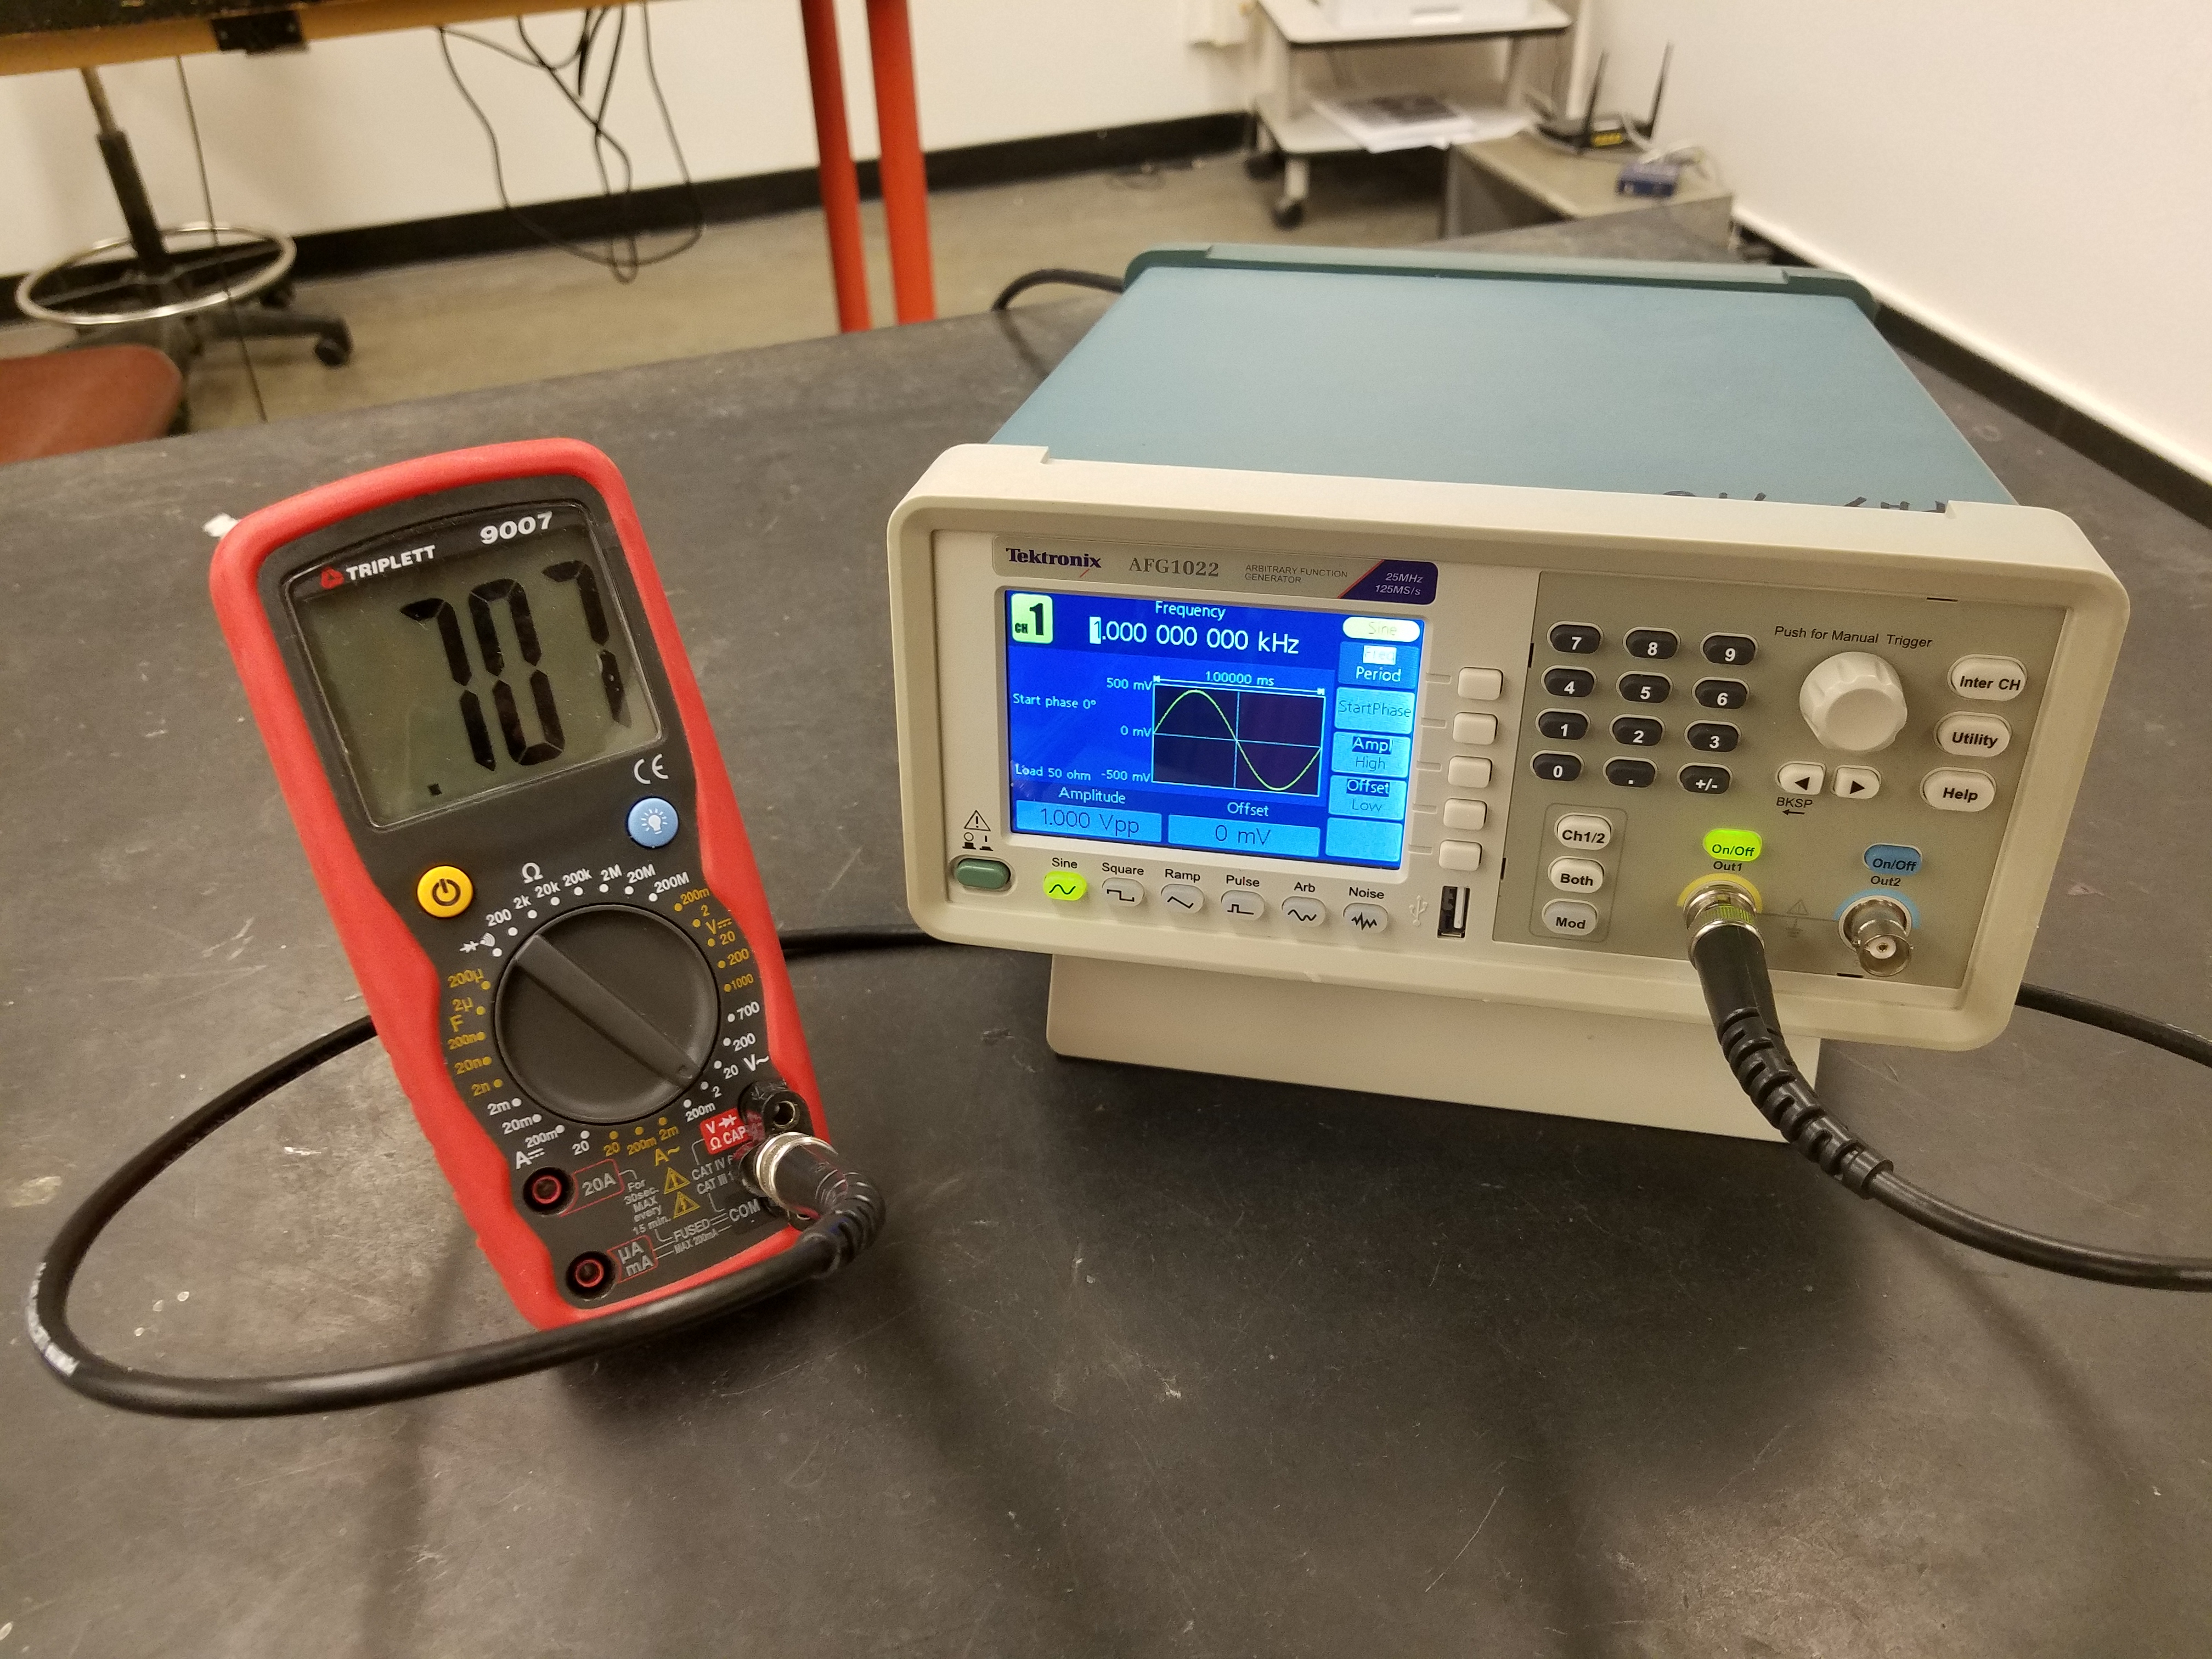
\includegraphics[width=0.45\textwidth]{figs/labs/lissajous/generator_dmm_setup.jpg} 
\caption{Connect the Channel 1 Output of your function generator directly to your DMM.}
\label{fig:dmm_setup}
\end{center}
\end{figure}

Connect the output of Channel 1 directly to the Voltage measurement
input of your Triplett 9007 DMM, using a BNC to banana plug adapter as
shown in Fig.~\ref{fig:dmm_setup}.  Turn on power to the function
generator.  Then set your function generator to the factory default:
\begin{displaymath}
\rm Utility\;Button \to System \to Set\;to\;Default \to Select.
\end{displaymath}
You must perform this step today for the instructions that follow to
make sense.  With shared equipment, it is essential to know how to
restore the factory default, in case another user has left the device
with strange settings.  You don't need to start with this step every
lab, but it is a fast way to recover when you encounter strange
behavior in your equipment.

The factory default settings are set to produce a Sine function with a
peak-to-peak voltage $v_{\rm pp} = 1.0~\rm V$ and a frequency $f=1~\rm
kHz$.  We'll leave that as is for now.  To turn on the output, push
the ``On/Off'' directly above the coaxial output for Channel 1, and
then ensure that the button is lit.

\begin{figure}[htbp]
\begin{center}
\begin{tabular}{ccc}
\begin{circuitikz}[line width=1pt]
\draw (0,0) coordinate(X) to[sinusoidal voltage source,bipoles/length=1.5cm] ++(0,2.0) 
to[R,l=$R_{\rm S}$] ++(0,2.0) to[short,-o] ++(1.0, 0) node[right]{B};
\draw (0.2,3.0) node[right] {$50~\rm \Omega$};
\draw (X) node[ground,yscale=2.0]{} to[short,-o] ++(1.0,0) node[right]{A};
\draw (0,-0.5) node[]{};
\end{circuitikz} &
\begin{circuitikz}[line width=1pt]
\draw (0,0) coordinate(X) to[short] ++(0,2.0) node[component]{V} to[short] ++(0,2.0) to[short,-o] ++(-1.0, 0) node[left]{B};
\draw (X) to[short,-o] ++(-1.0,0) node[left]{A};
\draw (0,-0.5) node[]{};
\end{circuitikz} &
\begin{circuitikz}[line width=1pt]
\draw (0,0) coordinate(X) to[short] ++(0,2.0) node[component]{V} to[short] ++(0,2.0) to[short] ++(-1.0, 0);
\draw (X) to[short,-*] ++(-1.0,0) coordinate(X) to[R,l=$R_L$] ++(0,4.0) to[short,*-o] ++(-1.0,0) node[left]{B};
\draw (X) to[short,-o] ++(-1.0,0) node[left]{A};
\draw (0,-0.5) node[]{};
\end{circuitikz} \\
(a) & (b) & (c) \\
\end{tabular}
\caption{Equivalent circuit for (a) your function generator, which includes a $50~\rm \Omega$ source resistance, and two typical terminations for a coaxial signal:  (b) infinite resistance voltmeter or scope, or (c) a terminating resistorin parallel.}
\label{fig:funccirc}
\end{center}
\end{figure}

Set your DMM to the $2~\rm V$ (AC) scale (the V with a squiggly line).
And you should now measure the AC voltage 
\begin{displaymath}
v_{\rm rms} = 0.707~\rm V \sim \frac{1}{\sqrt{2}}~\rm V
\end{displaymath}
However, recalling the relationships between the peak-to-peak voltage, the peak-voltage, and the RMS voltage of an AC sine wave:
\begin{displaymath}
v_{\rm pp} = 2 \, v_{\rm p} = 2 \sqrt{2} \, v_{\rm rms}
\end{displaymath}
we expect our function generator, set to $v_{\rm pp} = 1.0$, to produce output with:
\begin{displaymath}
v_{\rm rms} = \frac{v_{\rm pp}}{2\sqrt{2}} \sim 0.353~\rm V
\end{displaymath}
Clearly someone is lying to us!  In fact, we've encountered a very
common source of factor of two mistakes.  The equivalent circuit for
your function generator is shown in Fig.~\ref{fig:funccirc}a.  Notice
that it includes a $50~\rm \Omega$ source resistance in series with
the AC voltage produced by the function generator.  This internal
resistance is important for a number of reasons, most notably making
it impossible to short-circuit the output and destroy the
equipment!

In our setup, we've connected the function generator output directly
to your DMM, which has a very high input resistance, effectively
infinite, as shown in Fig.~\ref{fig:funccirc}b.  However, the standard
termination for coaxial cables is $50~\rm \Omega$, and the default
setting for your function generator expects the load shown in
Fig.~\ref{fig:funccirc}c with $R_{\rm L} = 50~\rm \Omega$.  In
this case, the internal resistance and load resistance form a voltage
divider, so that the output voltage $V_{\rm AB}$ seen by the user is
$1/2$ the internal AC voltage. The function generator is designed to
produce an internal AC voltage which is twice the value selected by
the user, so that the output voltage is precisely the value specified
by the user.  We are seeing twice our requested value, because we have
no load resistor, and so no voltage divider, and instead see the full
value of internal AC voltage.  To fix this discrepancy, we simply have
to configure our generator to expect a high load resistance at both
outputs:
\begin{eqnarray*}
{\rm Utility~Button \to CH1Load \to HighZ} \\
{\rm CH2Load \to HighZ}
\end{eqnarray*}
Press the ``Ch1/2'' button until you return to the Channel 1 menu.  Adjust the amplitude to $1~{\rm V}$ peak-to-peak by:
\begin{displaymath}
\rm Ampl \to 1 \to Vpp
\end{displaymath}
Your DMM should now read the expected value:
\begin{displaymath}
v_{\rm rms} \sim 0.353~\rm V
\end{displaymath}

Press the button next to Ampl a couple of times.  There is a slightly
annoying feature of your function generator which allows you to
specify either the Amplitude and Offset or the High and Low voltage
values.  So if you want to adjust the Amplitude, you have to press the
button next to Ampl until the Ampl label is highlighted.  Often you'll
end up setting the wrong value by mistake.  But in general, whatever
parameter is highlighted along the side of the screen is the parameter
which you can specify by either the knob or the key pad.  Keeping this
is mind, set your function generator to produce $1~\rm V$ RMS output:
\begin{displaymath}
\rm Ampl \to 1 \to Vrms.
\end{displaymath}
Now your DMM should also read a value quite close to one.

Now let's adjust the frequency. Highlight the frequency parameter by pressing the button next to the ``Freq'' option until it is highlighted:
\begin{displaymath}
\rm Freq \to 10 \to kHz.
\end{displaymath}
You can also adjust the selected parameter with the multipurpose knob.
Turn the multipurpose knob until the frequency is around $100~\rm kHz$
and observe what happens to your DMM measurement.  The reason your measurement is now inconsistent with the setting in the function generator, is that your DMM is only rated to $2~\rm kHz$.  It isn't intended for measuring
high-frequency AC signals.  Turn the frequency back down to $1~\rm kHz$.

Next highlight the Offset parameter on your function generator and
adjust it to $2~\rm V$.  This will add a DC offset to your function
generator output.  After settling down, the measured value of the AC
voltage on your DMM should be unchanged at $1~\rm V$.  Switch your DMM
to measure the DC voltage and you should now measure the $2~\rm V$ DC
offset.  Pay attention to the sign.  If you see a negative value, it
is because you installed your BNC-to-banana adapter incorrectly.
Notice that one side of the adapter has a small raised tab, indicating
which side connects to the coaxial cable shield.  The side with the
raised tab should be plugged into the Common socket.  Whether you got
lucky this time or not, change the orientation of the adapter a few
times and observe how the sign of the voltage changes, finally
plugging it back in with the correct orientation. Now adjust the DC
level with the multipurpose knob and observe the change on your DMM.
When satisfied, set the offset back to zero.

\section{Oscilloscope}

\begin{figure}[htbp]
\begin{center}
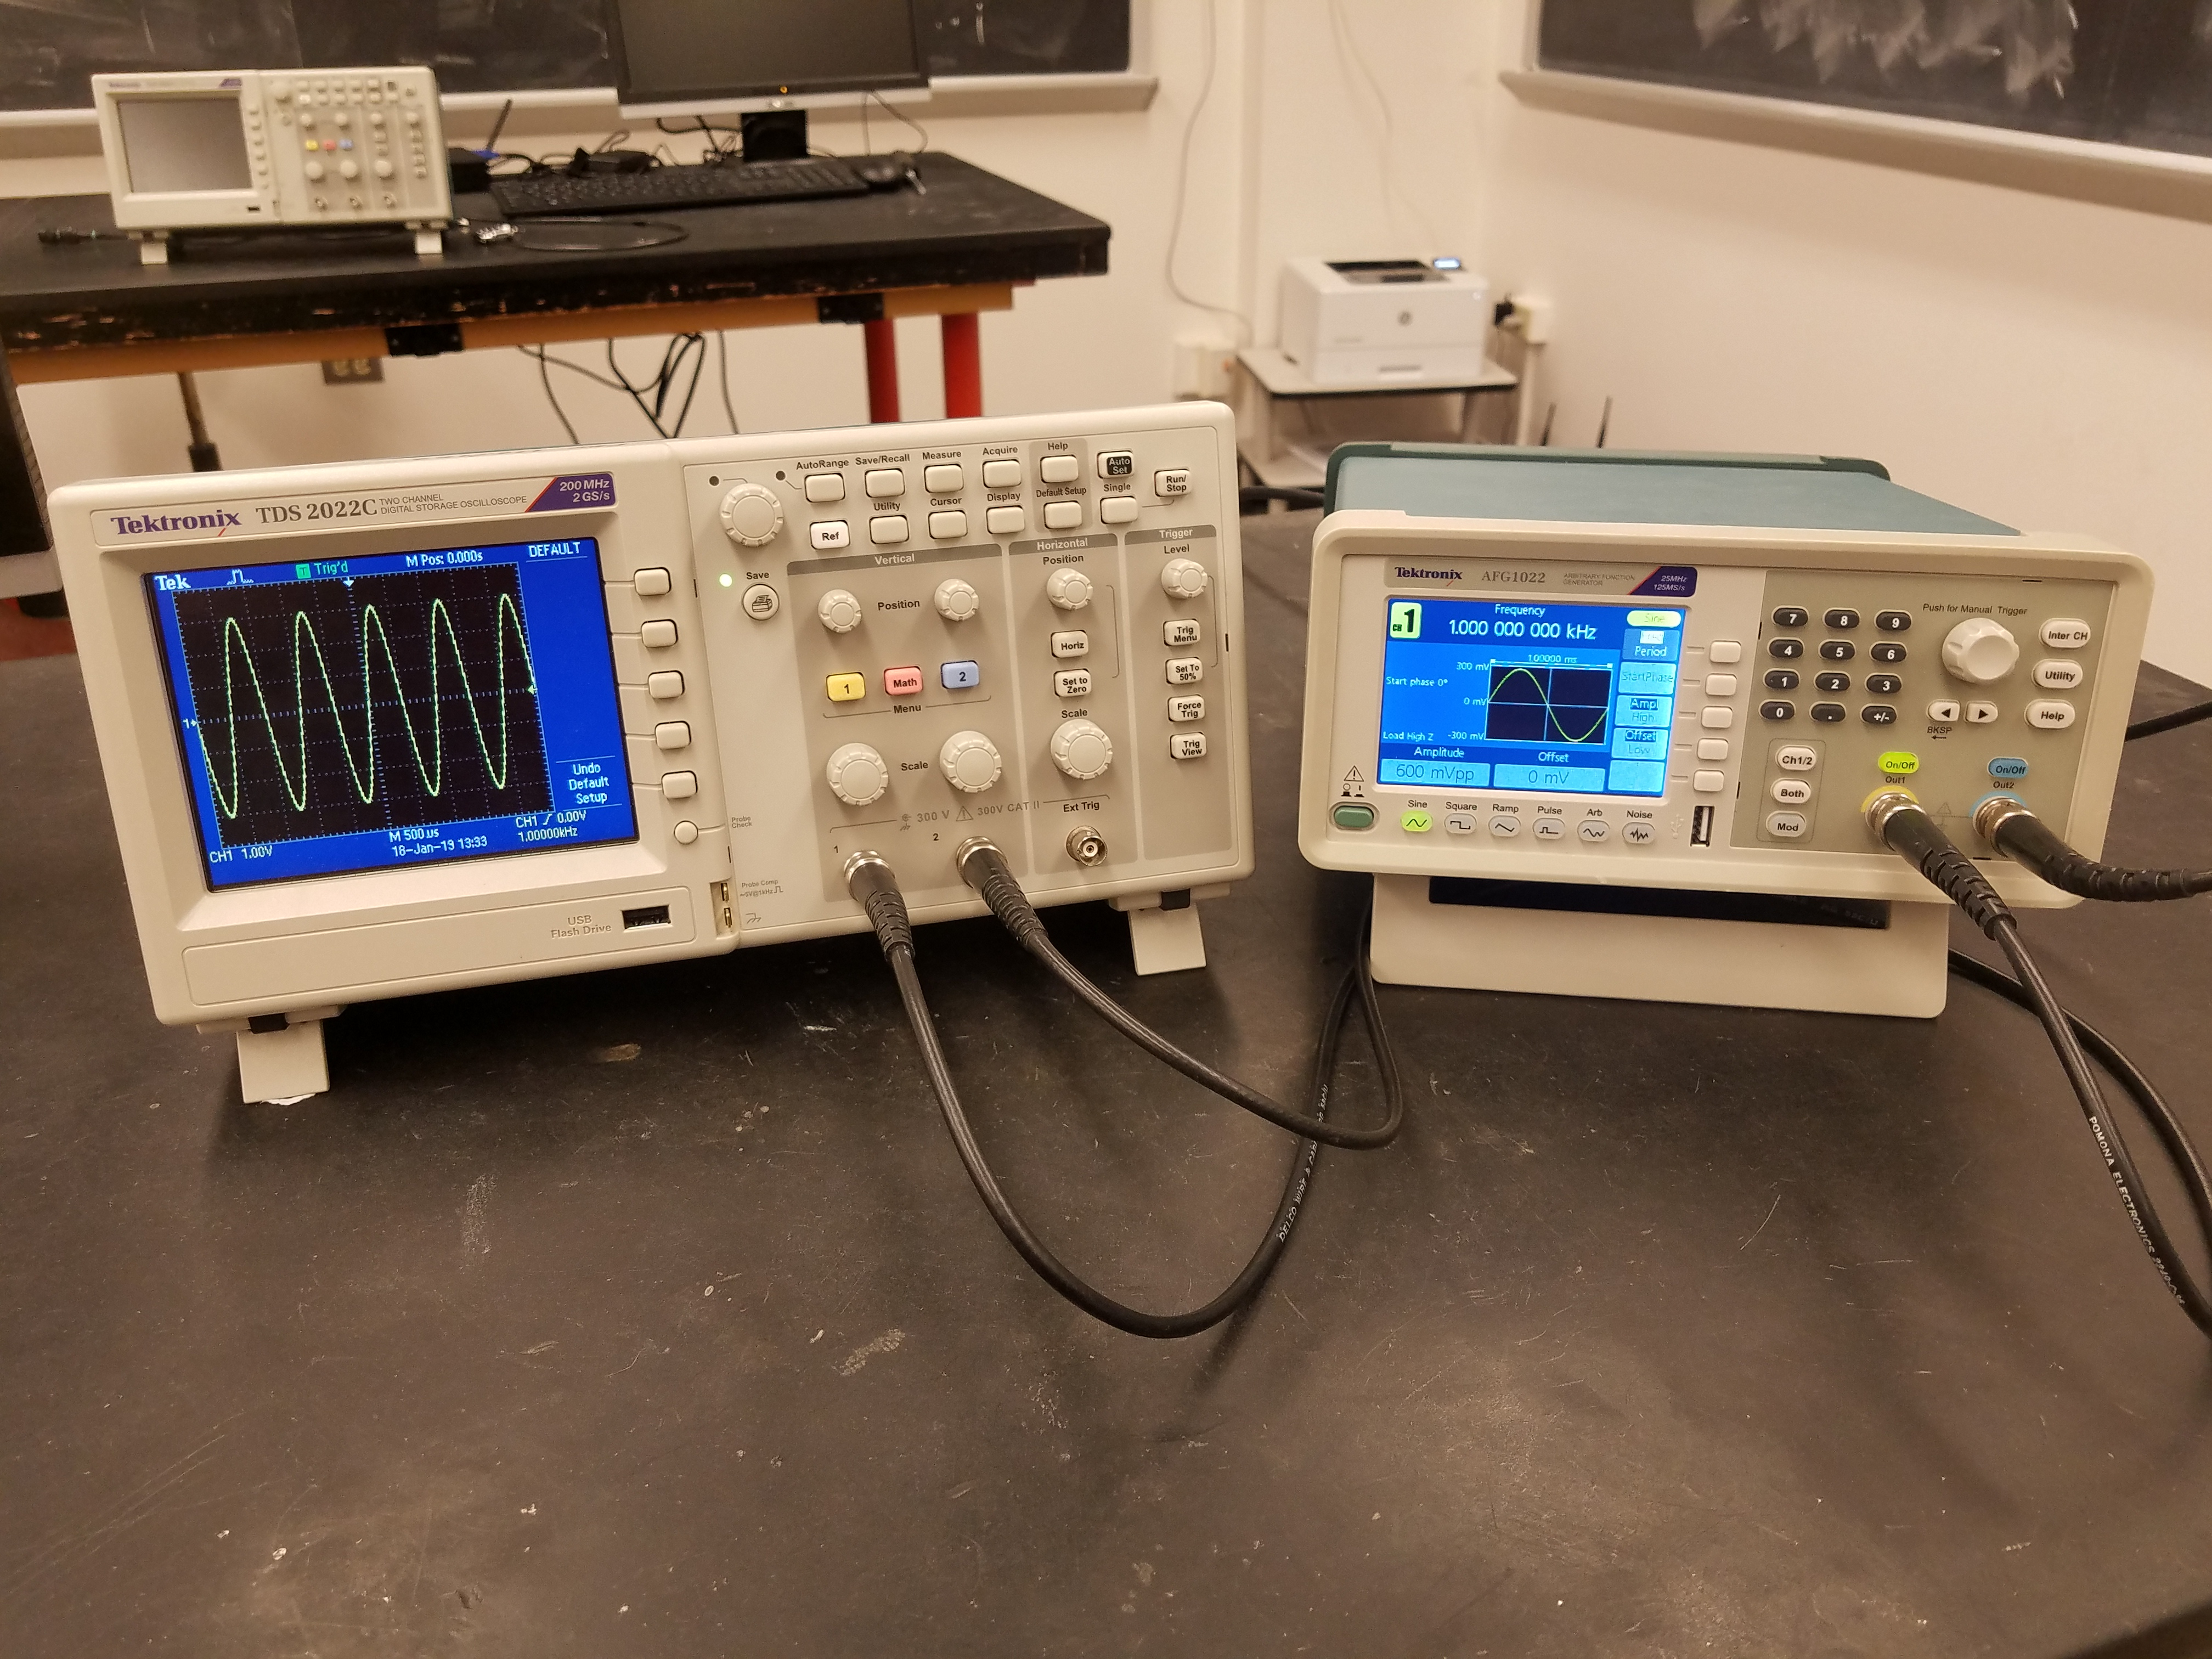
\includegraphics[width=0.45\textwidth]{figs/labs/lissajous/scope_setup.jpg} 
\caption{Connect the Channel 1 Output of your function generator directly to your DMM.}
\label{fig:scope_setup}
\end{center}
\end{figure}

Put your DMM aside.  Connect the Channel 1 output of your function
generator to the Channel 1 input of your digital oscilloscope.  Do the
same for Channel 2.  The setup is shown in Fig.~\ref{fig:scope_setup}.
Set your function generator to provide a $1~\rm kHz$ sine wave with
peak-to-peak voltage of $600~\rm mV$.  (A DC offset of zero is implied
unless otherwise stated) Press the ``Default Setup'' button on your
digital scope.  You should immediately observe a sine wave on your
Digital scope just as in Fig.~\ref{fig:scope_setup}.

Press the button labeled ``Square'' on your function generator to
change the output from a Sine wave to a square wave and observe the
waveform on your scope.  Do the same for the Ramp and
Noise functions.  Then return to a Sine wave.

Press the yellow button labeled ``1'' several times.  This button
turns on and off the display of channel 1, and brings up the Channel 1
parameter menu.  Notice that the voltage scale for Channel 1 is
indicated as $1.0~V$.  This means that the difference between each
pair of consecutive horizontal lines corresponds to $1~V$.  We say
``One volt per division''.  By counting divisions, you should be able
to see that your waveform has a peak-to-peak voltage of $6~\rm V$.
Yet your function generator is set to produce $600~\rm mV = 0.6~\rm
V$.  Clearly someone is lying to us!

\begin{figure}[htbp]
\begin{center}
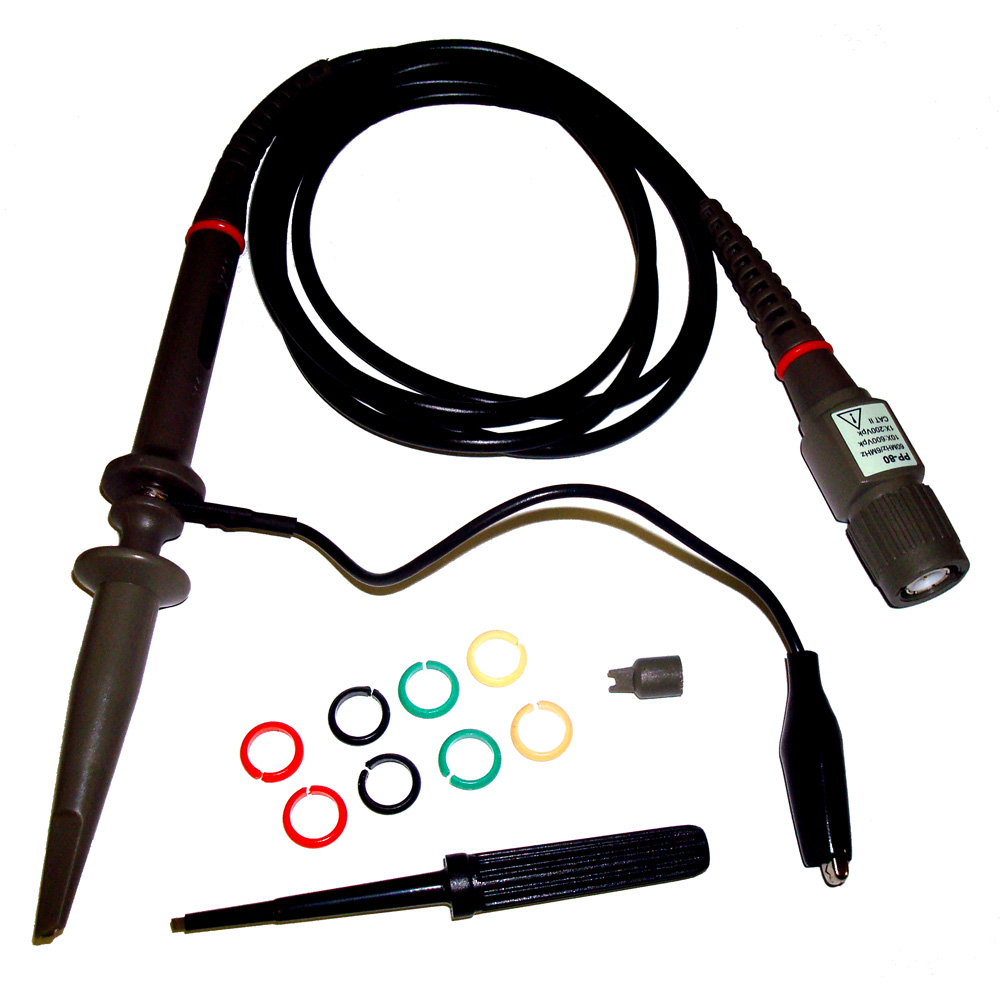
\includegraphics[width=0.45\textwidth]{figs/labs/lissajous/probe.jpg} 
\caption{An example scope probe.}
\label{fig:probe}
\end{center}
\end{figure}

Although we won't be using them in this lab, most sensitive
measurements with an oscilloscope are made using a scope probe, as
shown in Fig.~\ref{fig:probe}.  To protect the circuit being measured
from being effected by the insertion of the probe, there is usually a
large resistance in the probe.  This means that the oscilloscope
itself measures the output of a voltage divider, and the signal is
attenuated, most often by a factor of 10.  The oscilloscope simply
adjusts the voltage scale so that values you read are not attenuated.
To make consistent measurements, you simply have to make sure that the
oscilloscope is configured for the attenuation factor we are using.

In our case, we are connecting coaxial cables directly between the
oscilloscope and the function generator, and so their is no
attenuation.  But the default setup for the scope assumes that you are
using a probe with a $1/10$ attenuation, called a 10X probe.  Look at
the options next to the menu buttons and find the one that says
``Probe 10X Voltage''.  Press this menu button, and then press the
Attenuation button until it reads 1X, appropriate for a coaxial cable
with no attenuation factor.
\begin{figure}[htbp]
\begin{center}
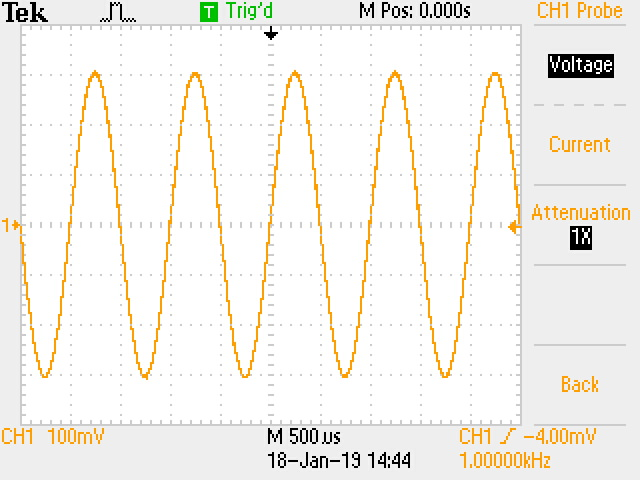
\includegraphics[width=0.45\textwidth]{figs/labs/lissajous/sine.jpg} 
\caption{Correctly scaled scope output.}
\label{fig:scopesine}
\end{center}
\end{figure}
The waveform is unchanged, but now the voltage scale is correctly set
to $100~\rm mV$.  And your signal now appears to be $600~\rm mV$,
consistent with the setting from your function generator, as shown in
Fig.~\ref{fig:scopesine}.  Next turn the knob labeled ``scale'' located
under the yellow channel ``1'' button.  Adjust this knob until the
scale for CH1 is listed as $200~\rm mV$ per division.  The apparent
size of the waveform will be reduced by a factor of two, because each
division is now $200~\rm mV$ and so your $600~\rm mV$ signal appears
three divisions high.

Next note that the function repeats every two divisions.  Since the
time scale is listed as $500~\rm \mu s$, the period is therefore $1~\rm
ms$, corresponding to a frequency of $1~\rm kHz$.  Adjust the time
scale, using the large knob in the Horizontal column, until the time
scale is $100~\rm \mu s$ per division.  This is still a $1~\rm kHz$
signal, but one period now takes up the entire display.

Using the multipurpose knob on your function generator, adjust the
frequency up to $10~\rm kHz$, and observe how the waveform changes.
Then adjust the voltage between about $100~\rm mV$ and $2~\rm V$
peak-to-peak.  When finished, leave the function generator producing a
$5~\rm kHz$ sine wave with $600~\rm mV$ peak-to-peak voltage.  Your
scope should remain at a voltage scale of $200~\rm mV$ and time scale
of $100~\rm \mu s$.  Next, set the DC offset of the signal on the function generator by pressing:
\begin{displaymath}
{\rm Offset \to 10 \to mV}
\end{displaymath}
Turn the multipurpose knob to adjust the DC offset between $-100~\rm
mV$ and $100~\rm mV$.  Your waveform will rise and fall on your
display.  By default, your scope includes the DC offset, but often this
is not what you want.  On your scope, press the button labeled
``Coupling DC'', until the DC becomes AC.  When AC coupled, the DC
component of your waveform is ignored.  When AC coupled, observe that
changing the DC offset on the function generator does not change the
position of the waveform.

You can adjust the position of the waveform using the small knobs
labeled ``Position'' to adjust the offset in vertical and horizontal.
Try this out.  To return a waveform to (0,0), notice that the offset
is displayed while you are turning the knob.

On your function generator, set the output to a $5~\rm V$ peak-to-peak
sine wave with frequency of $100~\rm kHz$.  Adjust the voltage scale
and time scale until you can clearly see the sine wave.

You now know most of the key features of your scope apart from the
trigger, which we'll leave for another day!

\section{Lissajous Figures}

\begin{figure}[htbp]
\begin{center}
\begin{tabular}{cc}
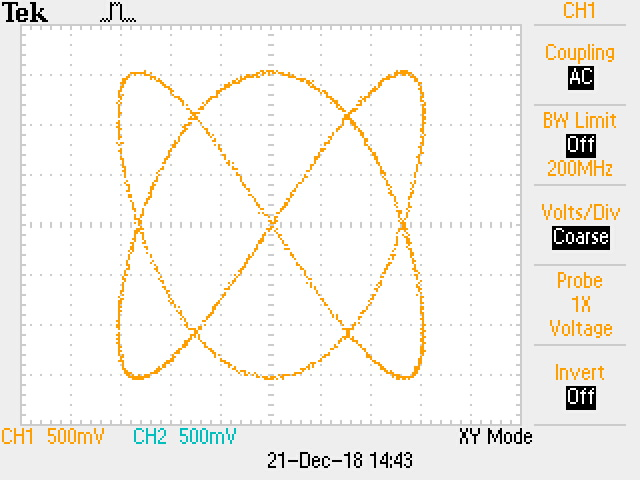
\includegraphics[width=0.45\textwidth]{figs/labs/lissajous/scope_lissajous.jpg} & 
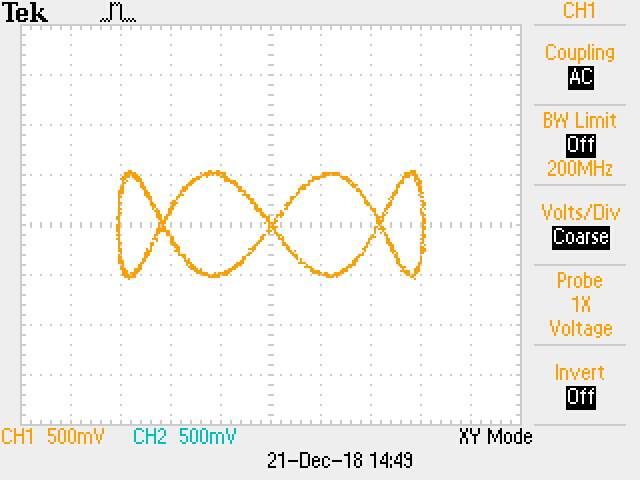
\includegraphics[width=0.45\textwidth]{figs/labs/lissajous/scope_crown.jpg} \\
(a) & (b) \\
\end{tabular}
\caption{Scope traces from Lissajous figures from settings for (a) start, and (b) crown.}
\label{fig:tracelissajous}
\end{center}
\end{figure}
Lissajous figures are the graph of system of two parameterized functions:
\begin{eqnarray*}
x &=& A_1 \sin(2 \pi f_1 t + \delta) \\
y &=& A_2 \sin(2 \pi f_2 t) 
\end{eqnarray*}
which produces a closed loop if the ratio $A_1 / A_2$ is rational.  The appearance of the figure is of a 3 dimensional knot with the viewing angle determined by the parameter $\delta$.  Two examples are shown in Fig.~\ref{fig:tracelissajous}.

To produce these figures on your scope, we'll need to use two
channels.  To begin, enable the output of both Channel 1 and Channel 2
on your function generator, and set them both to produce sine waves
with amplitude $3~\rm V$ peak-to-peak.  Adjust the frequency of
channel 1 to $2~\rm kHz$ and the channel 2 to $3~\rm kHz$.  Note that
you can switch between the Channel 1 and Channel 2 parameter menus
with the button labeled ``Ch1/2''.

\begin{figure}[htbp]
\begin{center}
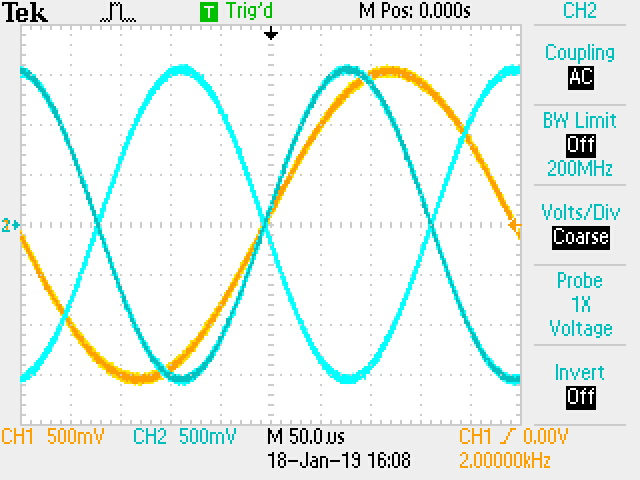
\includegraphics[width=0.45\textwidth]{figs/labs/lissajous/two_sine.jpg} 
\caption{Correctly scaled scope output.}
\label{fig:twosine}
\end{center}
\end{figure}

On your scope, switch to the Channel 2 parameter menu by pressing the
blue button labeled ``2''.  Set the coupling of Channel 2 to AC, and
probe attenuation to 1x, just as you did previously for Channel 1.
Next adjust the voltage scales of each channel to $500~\rm mV$ and set
the common time scale to something appropriate, so that you can view
both Sine waves on the display.  As shown in Fig.~\ref{fig:twosine},
you will see two versions of the Channel 2 output, inverted with
respect to each other, because the frequency of Channel 2 is 1.5 times
the frequency of Channel 1.  

The relative phase between the two output channels of your function
generator shifts whenever you adjust the frequency of one of the
signals.  For consistent results with offline plots and the scope
traces shown here, you'll need to align the phase of the two channels
every time you adjust the frequency on the function generator:
\begin{displaymath}
\rm Inter Ch button \to AlignPhase.
\end{displaymath}

Usually, scopes are used to display the inputs as a function of time.
In this case, the voltage level is along the $y$-axis, and time is the
$x$-axis.  This mode is called YT mode.  Occasionally, however, it is
useful to display things in XY mode.  In this mode, the $x$-axis is
used for the voltage of Channel 1 and the $y$-axis is used for the
voltage of Channel 2.  Each point on the curve represents a particular
point in time.  Switch to XY mode by pressing the Display button and
then pressing the button next to the Format menu item until the mode
is XY.  You should reproduce Fig.~\ref{fig:tracelissajous}a
exactly.  If not, check that you have aligned the phase as described
above and that frequencies are set correctly as in Table.

\begin{table}
\begin{center}
\caption{Settings for various Lissajous figures.}
\label{tbl:lissajous}
\begin{tabular}{llll}
pattern & $f_1~\rm(kHz)$ & $f_2~\rm(kHz)$ & $\delta_1$ \\
start & 2 & 3 & 0 \\
fish & 2 & 3 & $135^\circ$ \\
parabola & 1 & 2 & $45^\circ$ \\
lace & 13 & 12 & 0 \\
crown & $1~\rm kHz$ & $4~\rm kHz$ & 0 \\
\end{tabular}
\end{center}
\end{table}

Adjust the phase of Channel 2, under menu item StartPhase, until the
pattern collapses into a Fish pattern (or greek letter $\alpha$) at
135 degrees.  Save a scope trace by inserting your USB drive into the
scope and pressing the Save button.  Then produce the parabola and
lace patterns, according to the settings in Table~\ref{tbl:lissajous}, saving a scope
trace each time.  Remember to align the phase each time you change the
frequency.

Next, produce the crown pattern, shown in Fig.~\ref{fig:tracelissajous}b.
For the right proportions, adjust the amplitude of
Channel 2 to $1~\rm V$ peak-to-peak, leaving Channel 1 at $3~\rm V$
peak-to-peak.  Notice that as you adjust the phase of Channel 1, the
crown appears to rotate.  Adjust the frequency of Channel 2 to
$4.0002~\rm kHz$.  The crown should now appear to rotate constantly at
low speed.  This is a {\bf sign off} point in the lab.

\section{Analysis}

From the previous section, you should have scope traces for the fish,
parabola, and crown.  Reproduce each of these figures using scientific
python to draw the parameterized shape.  For
example. Fig.~\ref{fig:pythonlissajous}.

One way to approach this problem is to set the period to $1~\mu s$,
with fundamental angular frequency $\omega = 2 \pi~\rm kHz$.

One way to approach this problem is to set the period to $1~\mu s$.
The functions should be evaluated at 1000 discrete times within the
interval from 0 to $1~\mu s$.
\begin{verbatim}
     t = np.linspace(0,1,num=1000)
\end{verbatim}
Define a fundamental angular frequency $\omega_0 = 2 \pi~\rm kHz$:
\begin{verbatim}
     w = 2*np.pi
\end{verbatim}
With these definitions, we would define:
\begin{verbatim}
     x = np.sin(4*w*t)
\end{verbatim}
to obtain $x$ points corresponding to $f=4~\rm kHz$ sine function.

When plotting your curves, use:
\begin{verbatim}
       plt.axis('equal')
\end{verbatim}
to keep the unit aspect ratio used by your scope.
You can display your scope traces in python using the Image library like this:
\begin{verbatim}
       import Image

       image = Image.open('myscope.jpg')
       image.show()
\end{verbatim}

\begin{figure}[htbp]
\begin{center}
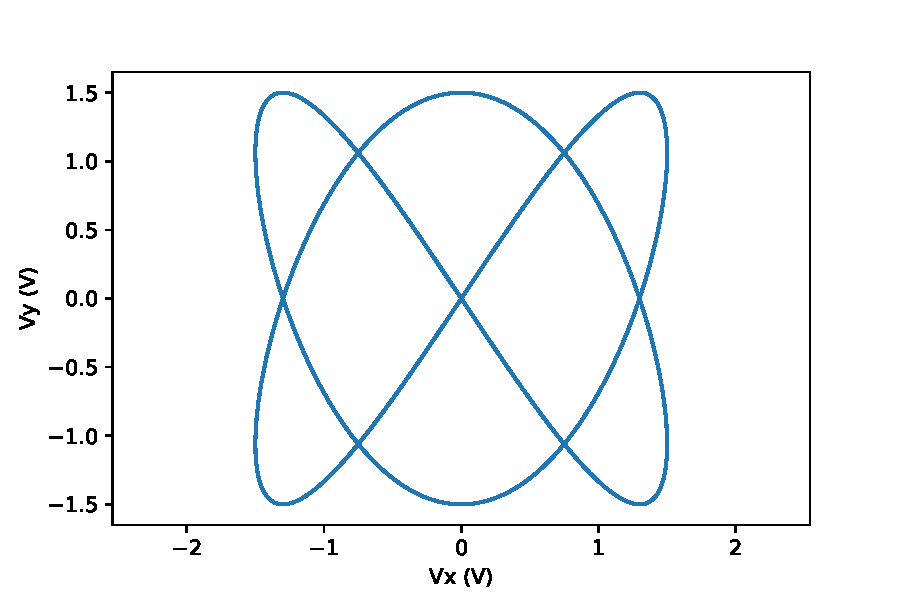
\includegraphics[width=0.45\textwidth]{figs/labs/lissajous/pythonlissajous.pdf} 
\caption{Lissajous curve constructed using Scientific Python corresponding to the scope trace in Fig.~\ref{fig:tracelissajous}a.}
\label{fig:pythonlissajous}
\end{center}
\end{figure}

